\textit{This section brings requirements to a greater level of detail making them usable by designers and testers. Examples:
Details on external interfaces
Precise specification of each function
Responses to abnormal situations
Detailed performance requirements
Database requirements
Design constraints
Specific attributes such as reliability, availability, security, portability}

\subsection{External Interfaces}
\label{requirements:interfaces}

	\subsubsection{User Interface}
	\label{requirements:interfaces:user}
        
        As described in section ?, this is how the final result could look like. Figure \ref{gui} is only a draft, trying to visualize how the integration into Tomboy can be accomplished.
        \begin{figure}[h]
          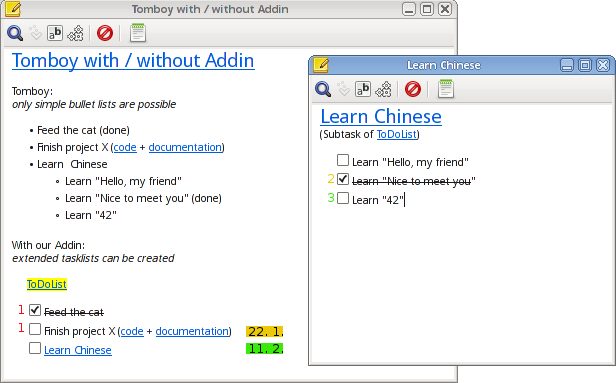
\includegraphics[width=\textwidth]{graphics/Screenshot_cropped_edited.png}
          \caption{GUI mockup}
          \label{gui}
        \end{figure}
        You can see the checkboxes for each of the todo items, along with some sample priorities to the left and some due dates to the right.
	
	\subsubsection{Hardware Interfaces}
	\label{requirements:interfaces:hardware}
	
	\subsubsection{Software Interfaces}
	\label{requirements:interfaces:software}

	\subsubsection{Communication Interfaces}
	\label{requirements:interfaces:communication}
	

\subsection{Functional Requirements}
\label{requirements:functional}


\subsection{Performance Requirements}
\label{requirements:performance}


\subsection{Design Constraints}
\label{requirements:constraints}


\subsection{Quality Requirements}
\label{requirements:quality}


\subsection{Other Requirements}
\label{requirements:other}
